\documentclass[1pt]{report}
\usepackage{multicol}
\setlength{\columnseprule}{0.2pt}
\usepackage[T1]{fontenc}
\usepackage[document]{ragged2e}
\usepackage[latin9]{inputenc}
\usepackage[left=.5cm, right=.5cm, top=.5cm, bottom=1cm]{geometry}
\usepackage{babel}
\usepackage{enumitem}
\usepackage{graphicx}
\usepackage{physymb}
\usepackage{verbatim}
\usepackage[linewidth=1pt]{mdframed}
\mdfsetup{skipabove=1pt,skipbelow=1pt}
\usepackage{subfig}
\begin{document}
\pagenumbering{gobble}
\begin{multicols}{3}
\begin{flushleft}

\begin{mdframed}
\textbf{Maxwell's Equations}\\
$\nabla\cdot E=\frac{1}{\epsilon_0}\rho$ | $\oint E\cdot da=\frac{1}{\epsilon_0}Q_{enc}$\\
$\nabla\cdot B=0$\\
$\nabla\times E=-\frac{\delta B}{\delta t}$ | $\oint E\cdot dl=-\frac{d\phi}{dt}$\\
$\nabla\times B=\mu_0J+\mu_0\epsilon_0\frac{\delta E}{\delta t}$\\
$\oint B\cdot dl=\mu_0 I_{enc}+\mu_0\epsilon_0\int(\frac{\delta E}{\delta t})\cdot da$\\
\end{mdframed}

\textbf{Vector Analysis}\\
$A\times B=(A_yB_z-A_zB_y)\hat{x}+(A_zB_x-A_xB_z)\hat{y}+(A_xB_y-A_yB_x)\hat{z}$\\
$A\times B=(A_\phi B_z-A_zB_\phi )\hat{r}+(A_zB_r-A_rB_z)\hat{\phi }+(A_rB_\phi -A_\phi B_r)\hat{z}$\\
$A\times B=(A_\theta B_\phi -A_\phi B_\theta )\hat{r}+(A_\phi B_r-A_rB_\phi)\hat{\theta }+(A_rB_\theta -A_\theta B_r)\hat{\phi}$\\
$\nabla T=(\hat{x}\frac{\delta}{\delta x}+\hat{y}\frac{\delta}{\delta y}+\hat{z}\frac{\delta}{\delta z})$\\
$r=\sqrt[]{x^2+y^2+z^2}$\\
$\hat{r}=\frac{\textbf{r}}{r}=\frac{x\hat{x}+y\hat{y}+z\hat{z}}{\sqrt[]{x^2+y^2+z^2}}$\\
$\pmb{\scriptr}=\textbf{r-r'}$ $_{r'=SourcePoint,r=FieldPoint}$\\
$\hat{{\pmb{\scriptr}}}=\frac{{\pmb{\scriptr}}}{{\pmb{\scriptr}}}=\frac{r-r'}{|r-r'|}$\\
$f(x)\delta(x)=f(0)\delta(x)$\\
$\int_{_\infty}^{\infty}f(x)\delta(x-a)dx=f(a)$\\
$\delta(kx)=\frac{1}{|k|}\delta(x)$\\

\noindent\rule[0.5ex]{\linewidth}{1pt}

\textbf{Electrostatics}\\
$F=\frac{1}{4\pi\epsilon_0}\frac{qQ}{\pmb{\scriptr}^2}$\\
$F=QE$\\
$E(r)=\frac{1}{4\pi\epsilon_0}\int\frac{\rho(r')}{\pmb{\scriptr}^2}\hat{\pmb{\scriptr}}d\tau'$\\
$E_{wire}=\frac{1}{4\pi\epsilon_0}\frac{2\lambda}{r}$\\
$E_{point}=\frac{1}{4\pi\epsilon_0}\frac{q}{r^2}$\\
$E=-\nabla V$\\
$E^{\parallel}_{above}=E^{\parallel}_{below}$\\
$E^{\perp}_{above}-E^{\perp}_{below}=\frac{1}{\epsilon_0}\sigma$\\
$E_{dip}(r,\theta)=\frac{\rho}{4\pi\epsilon_0r^3}(2cos\theta\hat{r}+sin\theta\hat{\theta})$
$E_{dip}=\frac{1}{4\pi\epsilon_0}\frac{1}{r^3}[3(p\cdot\hat{r})\hat{r}-p]$\\
$\phi_E=\int_s E\cdot da$ $_{\phi=Flux}$\\
$\oint E\cdot dl=0$\\
$\nabla\times E=0$\\
$V(r)\equiv-\int_a^b E\cdot dl$\\
$V(r)=\frac{1}{4\pi\epsilon_0}\int\frac{\rho(r')}{\pmb{\scriptr}}d\tau'$\\
$V_{point}=\frac{1}{4\pi\epsilon_0}\frac{q}{r}$\\
$\nabla^2V=-\frac{\rho}{\epsilon_0}$ $_{Poisson'sEquation}$\\
$V_{above}-V_{below}=-\oint_a^b E\cdot dl$\\
$W=\int_a^b F\cdot dl=\frac{\epsilon_0}{2}\int E^2 d\tau$\\
$W=\frac{1}{2}CV^2$\\
$C\equiv\frac{Q}{V}$\\
$C=4\pi\epsilon_0\frac{ab}{(b-a)}$ $_{CocentricShells}$\\

\noindent\rule[0.5ex]{\linewidth}{1pt}

\textbf{Potentials}\\
\textit{First Uniqueness Theorem:}
The solution to Laplace equation in some volume \textit{V} is uniquely determined if V is specified on the boundary surface \textit{S}\\
\textit{Second Uniqueness Theorem:}\\
In a volume \textit{V} surrounded by a conductors and containing a specified charge density \textit{$\rho$}, the electric field is uniquely determined if the \textit{total charge} on each conductor is given. (The region as a whole can be bounded by another conductor or else unbounded)\\
\textit{Method of Images}\\
\textbf{$\cdot$} Replace the conducting plane with a mirror image charge\\
\textbf{$\cdot$} Use Gausss law on each charge in isolation\\
\textbf{$\cdot$} Sum up the electric field contribution from each charge\\
$V(x,y)=(Ae^{kx}+B^{-kx})(Csin\textit{ky}+Dcos\textit{ky})$
$V(r,\theta)=\sum_{l=0}^{\infty}(A_lr^l+\frac{B_l}{r^{l+1}})P_l(cos\theta)$\\
$V_{mon}=\frac{1}{4\pi\epsilon_0}\frac{Q}{r}$\\
$V_{dip}\approx\frac{1}{4\pi\epsilon_0}\frac{qdcos\theta}{r^2}$ $_{d=DipoleDistance}$\\
$V_{dip}=\frac{1}{4\pi\epsilon_0}\frac{p\cdot\hat{r}}{r^2}$ $_{p=DipoleMoment}$\\
$p\equiv\int r'\rho(r')d\tau'=\sum_{i=1}^{n}q_ir_i'$\\
$P_0(x) = 1$\\
$P_1(x) = x$\\
$P_2(x) = \frac{1}{2}(3x^2 - 1)$\\
$P_3(x) = \frac{1}{2}(5x^3-3x)$\\
$E_{dip}(r,\theta)=\frac{\rho}{4\pi\epsilon_0r^3}(2cos\theta\hat{r}+sin\theta\hat{\theta})$
$E_{dip}=\frac{1}{4\pi\epsilon_0}\frac{1}{r^3}[3(p\cdot\hat{r})\hat{r}-p]$\\

\noindent\rule[0.5ex]{\linewidth}{1pt}

\textbf{Electric Fields In Matter}\\
$p=\alpha E$ $_{p=DipoleMoment,\alpha=Polarizability}$\\
$N_{dip}=p\times E$ $_{N=Torque}$\\
$F_{dip}=(p\cdot\nabla)E$\\
$U_{dip}=-p\cdot E$\\
$P\equiv _{DipoleMomentPerUnitVolume/Polarization}$\\
$\sigma_b\equiv P\cdot \hat{n}$ $_{\sigma_b=BoundSurfaceCharge}$\\
$\rho_b\equiv -\nabla\cdot P$ $_{\rho_b=BoundVolumeCharge}$\\
$D\equiv\epsilon_0 E+P$ $_{D=ElectricDisplacement}$\\
$\nabla\cdot D=\rho_f$\\ 
$\oint D\cdot da=Q_{f_{enc}}$\\
$D=\epsilon E$\\
$\epsilon\equiv\epsilon_0(1+\chi_e)$ $_{\chi_e=ElectricSusceptability}$\\
$\epsilon_r\equiv1+\chi_e=\frac{\epsilon}{\epsilon_0}$ $_{\epsilon_r=RelativePermattivity}$\\
$C=\epsilon_rC_{vac}$ $_{ForLinearDialectric}$\\

\noindent\rule[0.5ex]{\linewidth}{1pt}

\textbf{Magnetostatics}\\
Magnetic forces do no work.\\
Stationary charges $\rightarrow$ Electrostatics\\
Steady currents $\rightarrow$ Magnetostatics\\
$F_{mag}=Q(v\times B)$\\
$F_{mag}=\int I(dl\times B)$\\
$K=\frac{dI}{dl_\perp}=\sigma v$ $_{(K=Surface Current Density)}$\\
$J=\frac{dI}{da_\perp}=\rho v$ $_{(J=Volume Current Density)}$\\
$J=\frac{1}{\mu_0}(\nabla\times B)$\\
$\nabla\cdot J=-\frac{\delta\rho}{\delta t}$\\
$\nabla\times B=\mu_0J$\\
$\oint B\cdot dl=\mu_0 I_{enc}$\\
$B=\nabla\times A$ $_{(A=Vector Potential)}$\\
$\nabla\cdot A=0$\\
$\nabla^2A=-\mu_0J$\\
$A(r)=\frac{\mu_0}{4\pi}\int\frac{J(r')}{{\pmb{\scriptr}}}d\tau'$\\
$A_{above}=A_{below}$\\
$A_{dip}(r)=\frac{\mu_0}{4\pi}\frac{m\times\hat{r}}{r^2}$\\
$B^{\perp}_{above}=B^{\perp}_{below}$\\
$B^{\parallel}_{above}-B^{\parallel}_{below}=\mu_0K$\\
$B_{above}-B_{below}=\mu_0(K\times\hat{n})$\\
$m=I\int da=Ia$ $_{(m=MagneticDipoleMoment)}$\\
$B_{dip}(r)=\frac{\mu_0}{4\pi}\lbrack 3(m\cdot\hat{r})\hat{r}-m\rbrack$\\
$B_{line}=\frac{\mu_0I}{4\pi s}(sin\theta_2-sin\theta_1)$\\
$B_{loop}=\frac{\mu_0 I}{2r}$\\
$B_{wire}=\frac{\mu_0 I}{2\pi r}$\\
$B_{solenoid}=\mu_0nI$\\
$J_b=\nabla\times M$\\
$K_b=M\times\hat{n}$\\

\noindent\rule[0.5ex]{\linewidth}{1pt}

\textbf{Magnetic Fields in Matter}\\
$N=m\times b$ $_{N=Torque}$\\
$F_{loop}=\nabla(m\cdot B)$\\
$J_b=\nabla\times M$ $_{J_b=VolumeBoundCurrent}$\\
$K_b=M\times\hat{n}$ $_{K_b=SurfaceBoundCurrent}$\\
$H\equiv\frac{1}{\mu_0}B-M$\\
$\nabla\times H=J_f$ | $\oint H\cdot dl=I_{f_{enc}}$\\
$\nabla\cdot H=-\nabla\cdot M$\\
$M\equiv _{MagneticDipoleMoment/Magnetization}$\\
$M=\chi_m H$ $_{\chi_m=MagneticSusceptibility}$\\
$B=\mu H$\\
$\mu\equiv\mu_0 (1+\chi_m)$\\
$U_{dip}=-m\cdot B$\\

\noindent\rule[0.5ex]{\linewidth}{1pt}

\textbf{Electrodynamics}\\
$F=ma=qE$\\
$J=\sigma(E+v\times B)$ $_{\sigma=Conductivity}$\\
$J=\sigma E$ $_{Ohm's Law}$\\
$J_d=\epsilon_0\frac{\delta E}{\delta t}$\\
$I=\sigma\int E\cdot da$\\
$P=VI=I^2R$\\
$V=IR$\\
$\tau=RC$\\
$\varepsilon\equiv\oint f\cdot dl=\oint f_s\cdot dl$ $_{\varepsilon=ElectromotiveForce}$\\
$\varepsilon=-\frac{d\Phi}{dt}$\\
$\varepsilon=IR$\\
A Changing magnetic field induces an electric field\\
Nature abhors a change in flux\\
$F_{mag}=\int I(dl\times B)$\\
$F_{mag}=Q(v\times B)$\\
$\Phi=LI$ $_{L=SelfInductance}$\\
$\varepsilon=-L\frac{dI}{dt}$\\
$W=\frac{1}{2}LI^2$\\
$W=\frac{1}{2\mu_0}\int_{all space} B^2d\tau$\\

\noindent\rule[0.5ex]{\linewidth}{1pt}

\textbf{Conservation Laws}\\
$\frac{\delta\rho}{\delta t}=-\nabla\cdot J$\\
$u=\frac{1}{2}(\epsilon_0E^2+\frac{1}{\mu_0}B^2)$ $_{u=EnergyPerVolume}$\\
$S\equiv\frac{1}{\mu_0}(E\times B)$ $_{S=PoyntingVector}$\\
$P=\int S\cdot da$\\

\noindent\rule[0.5ex]{\linewidth}{1pt}

\textbf{Electromagnetic Waves}\\
$\omega=2\pi v=kv$\\
$\frac{\delta^2 f}{\delta z^2}=\frac{1}{v^2}\frac{\delta^2 f}{\delta t^2}$\\
$\nabla^2E=\mu_0\epsilon_0\frac{\delta^2E}{\delta t^2}$\\
$\nabla^2B=\mu_0\epsilon_0\frac{\delta^2B}{\delta t^2}$\\
$E(z,t)=E_0cos(kz-\omega t+\delta)\hat{x}$\\
$B(z,t)=\frac{1}{c}E_0cos(kz-\omega t+\delta)\hat{y}$\\
$\tilde{E}(r,t)=\tilde{E}_0e^{i(k\cdot r-\omega t)}\hat{n}$\\
$\tilde{B}(r,t)=\frac{1}{c}\tilde{E}_0e^{i(k\cdot r-\omega t)}(\hat{k}\times\hat{n})=\frac{1}{c}\hat{k}\times\tilde{E}$\\

\end{flushleft}
\end{multicols}
\begin{figure}[h]
\centering
\subfloat{\includegraphics[scale=.5]{Griffiths.png}}
\qquad
\subfloat{\includegraphics[scale=.5]{Griffiths2.png}}




\fbox{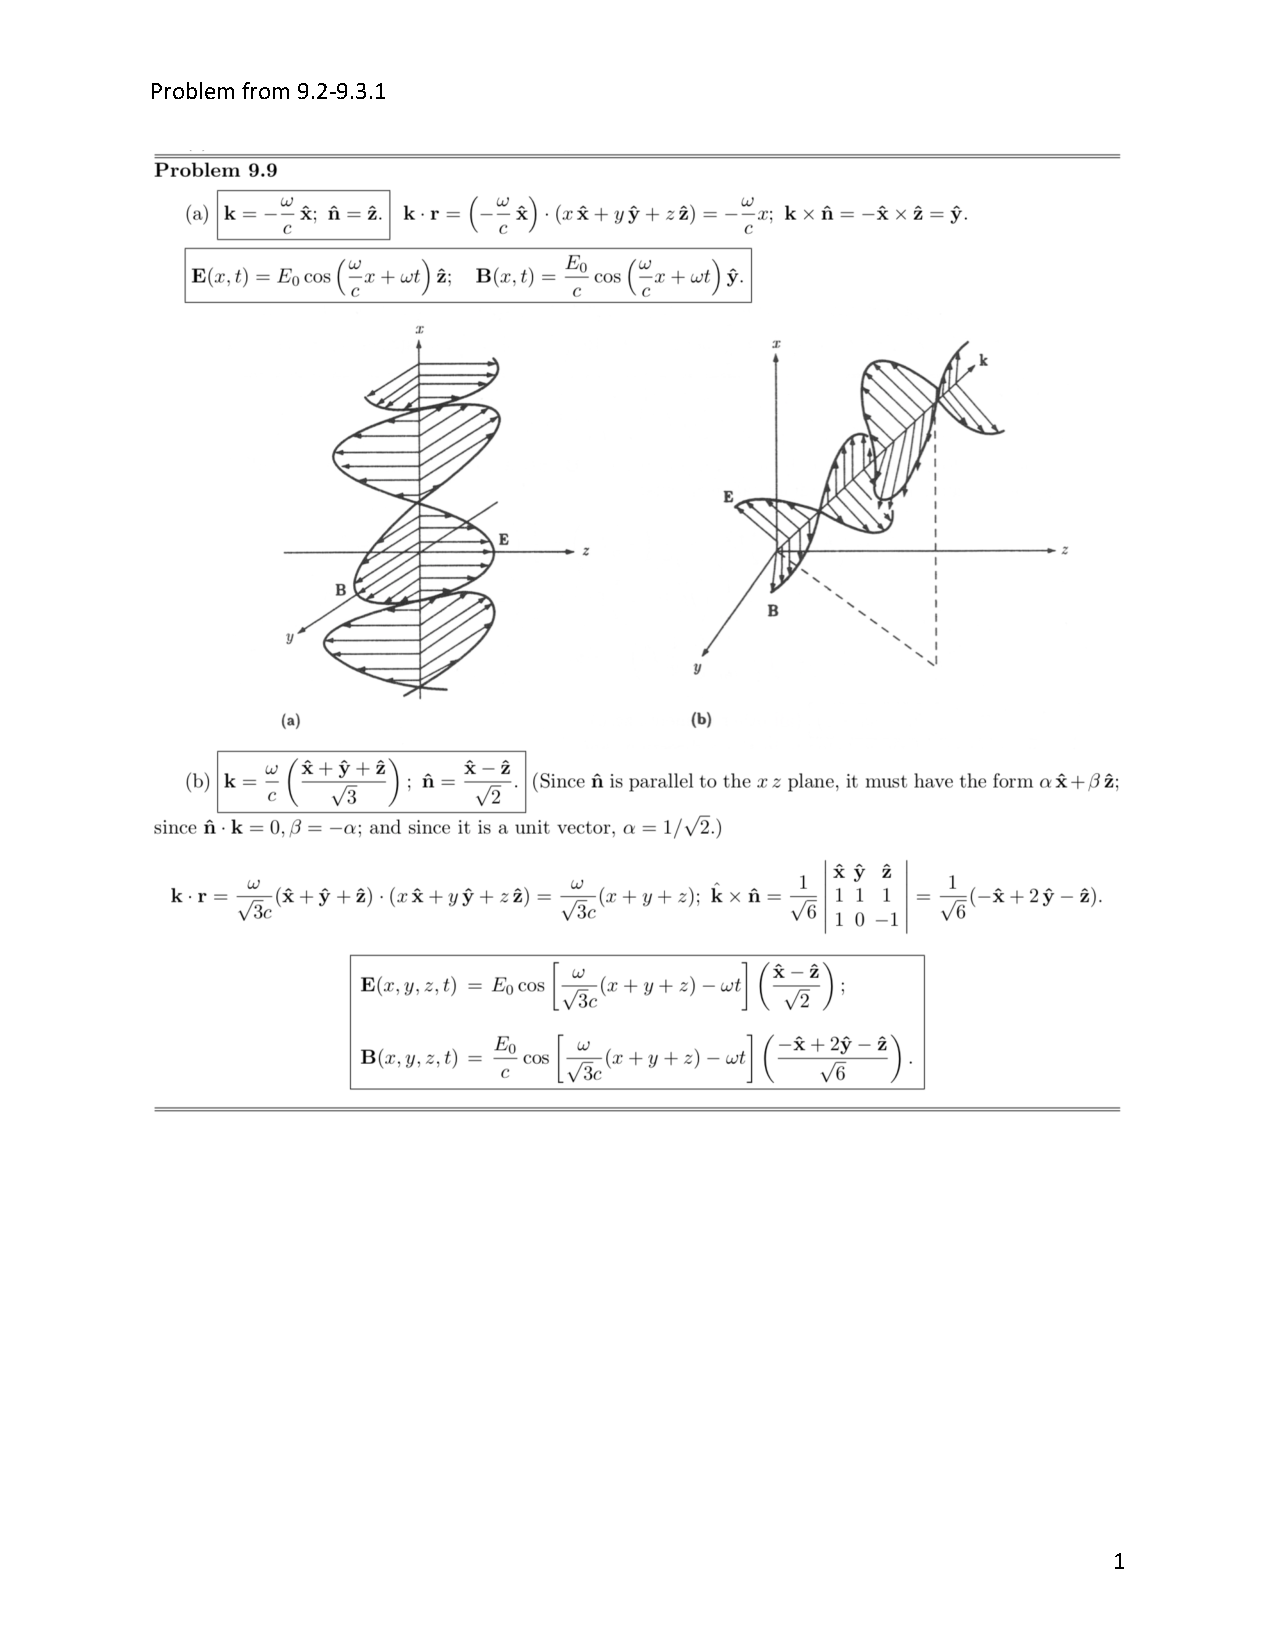
\includegraphics[trim=2.5cm 6.5cm 2.5cm 2.5cm, clip, scale=.5]{HW32.pdf}}
\fbox{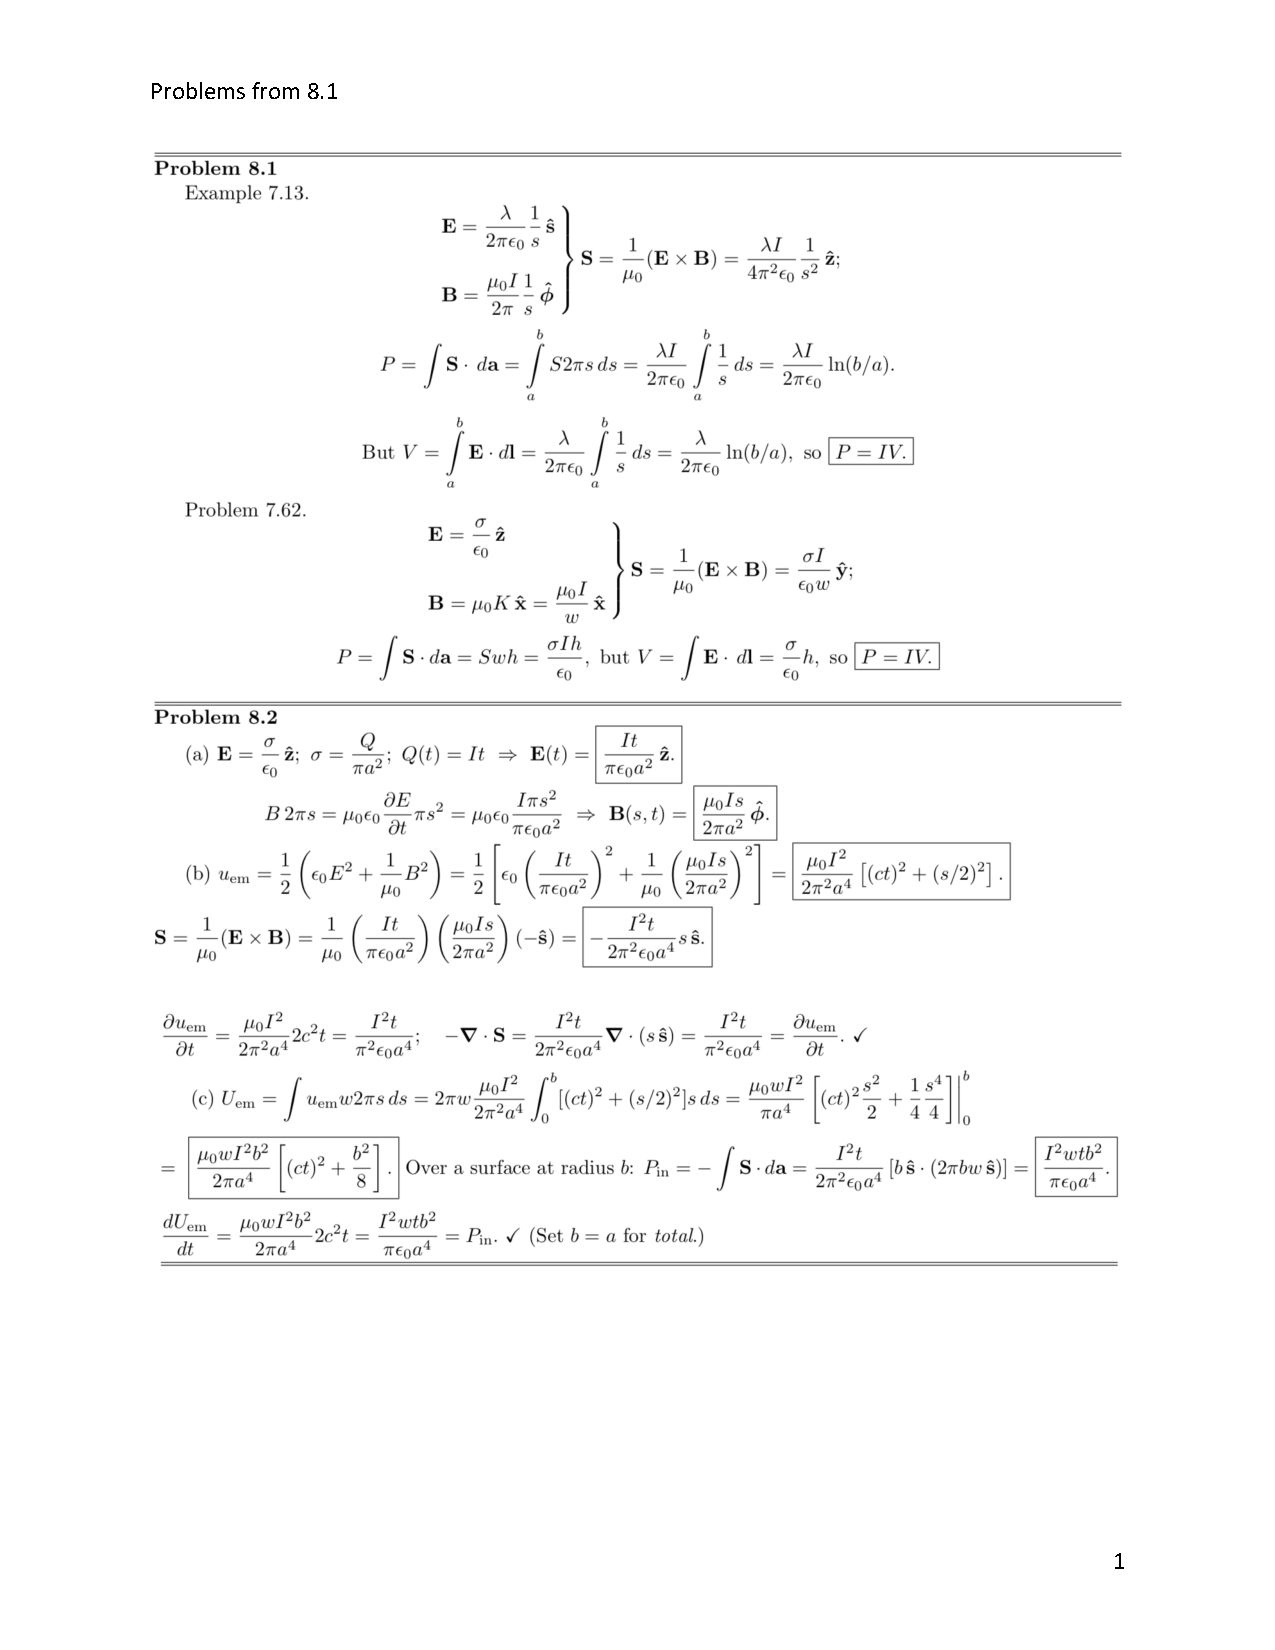
\includegraphics[trim=2.5cm 6.5cm 2.5cm 2.5cm, clip, scale=.5]{HW31.pdf}}

\fbox{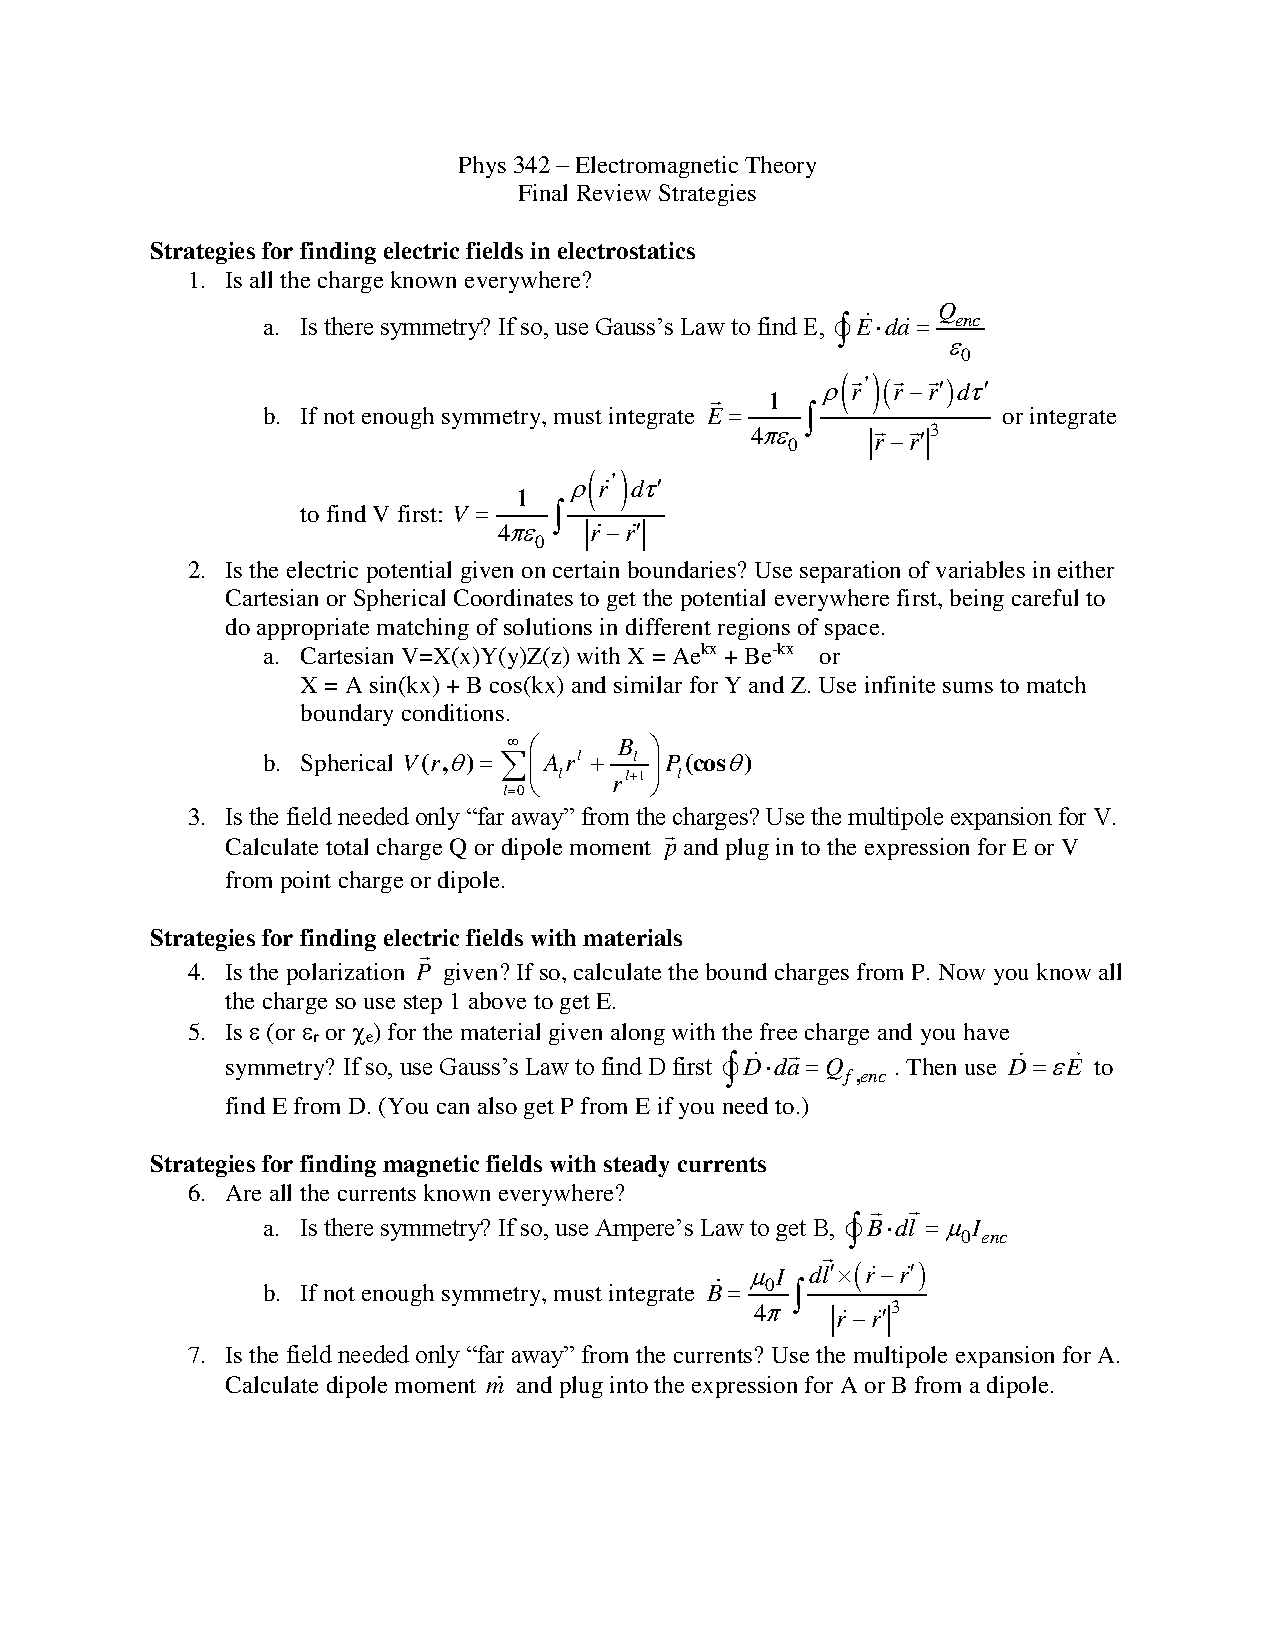
\includegraphics[trim=2.5cm 4cm 2.5cm 2.5cm, scale=.5]{Final.pdf}}
\fbox{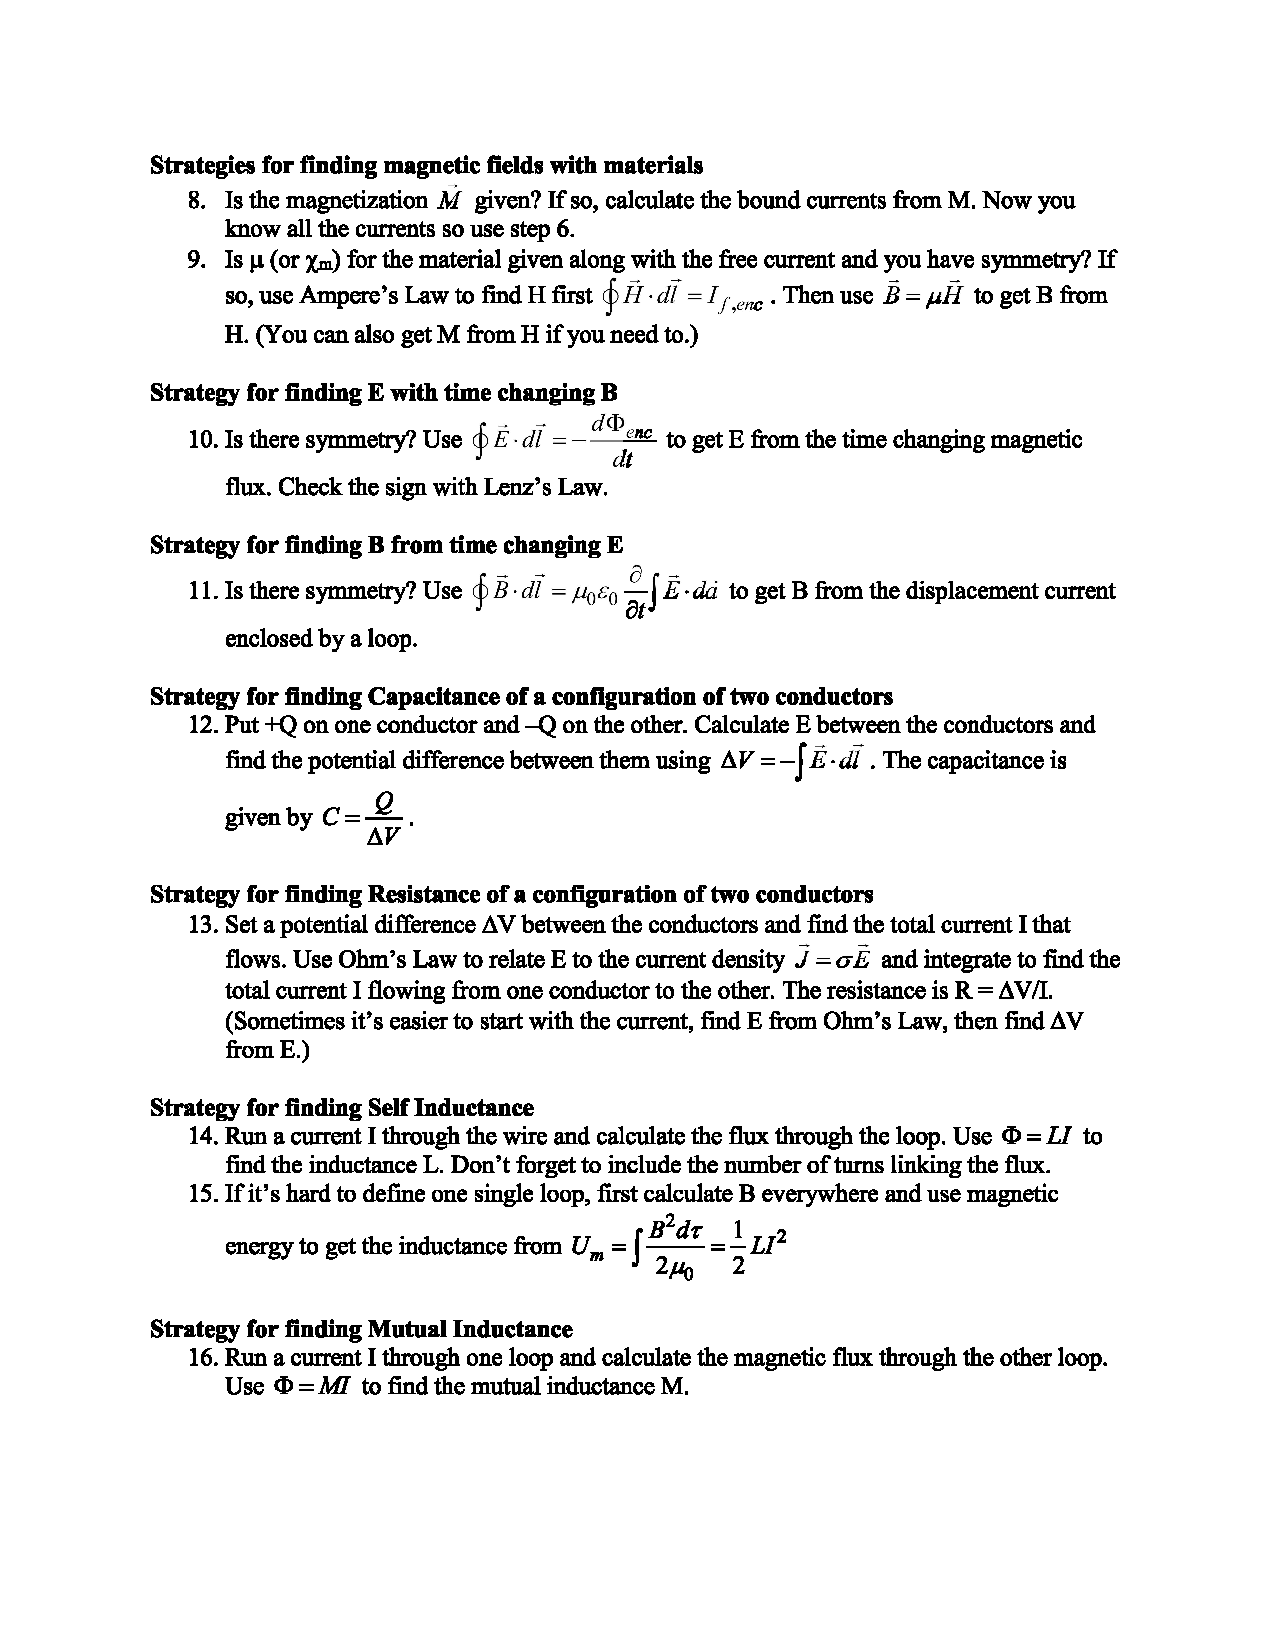
\includegraphics[trim=2.5cm 4cm 2.5cm 2.5cm, scale=.5]{Final2.pdf}}
\end{figure}

\bigskip
\bigskip
\bigskip





















\begin{comment}
$\oint_S {E_n dA = \frac{1}{{\varepsilon _0 }}} Q_{inside}$
\linebreak
$\nabla\cdot E=\frac{1}{\epsilon_0}\rho$|$V(r)=-\int^rE\cdot dl$
\linebreak
$E=-\nabla V$|$C=\frac{Q}{V}$
\linebreak
$W=\frac{1}{2}CV^2$|$W=\frac{\epsilon_0}{2}\int E^2d\tau$
\linebreak
$V(r)=\frac{1}{4\pi\epsilon_0}\int\frac{\rho(r)}{r_s}d\tau$
\linebreak
Potential is continuous at boundaries 
\textbf{Method of Images}
\begin{itemize}[noitemsep]
\item Replace the conducting plane with a mirror image charge
\item Use Gausss law on each charge in isolation
\item Sum up the electric field contribution from each charge
\end{itemize}
Poisson's equation:
$\nabla^2V=-\frac{1}{\epsilon_0}\rho$
\linebreak
Laplace's equation:
$\nabla^2V=0$
\linebreak
Laplace's equation in Cartesian:
$\frac{\delta^2V}{\delta x^2}\frac{\delta^2V}{\delta y^2}\frac{\delta^2V}{\delta z^2}=0$
\linebreak
Converted to PDE
\linebreak
$V(x,y)=(Ae^{kx}+B^{-kx})(Csin(ky)+Dcos(ky))$
Laplace's equation is true if $\rho$ is zero
\linebreak
\textbf{First Uniqueness Theorem:}
The solution to Laplace equation in some volume \textit{V} is uniquely determined if V is specified on the boundary surface \textit{S}
\textbf{Corollary:}
The potential in a volume \textit{V} is uniquely determined if (a) the charge density throughout the egion, and (b) the value of V on all boundaries, are specified. 
\textbf{Second Uniqueness Theorem:}
In a volume \textit{V} surrounded by a conductors and containing a specified charge density \textit{$\rho$}, the electric field is uniquely determined if the \textit{total charge} on each conductor is given. (The region as a whole can be bounded by another conductor or else unbounded)
\textbf{Fourier s Trick}
$V_0(y) = \sum_{n=1}^{\infty} C_n \sin \left(\frac{n \pi y}{a} \right)$
\linebreak
$V_0(y) \sin \left(\frac{n' \pi y}{a} \right) =\sum_{n=1}^{\infty} C_n \sin \left(\frac{n \pi y}{a} \right)\sin \left(\frac{n' \pi y}{a} \right)$
\linebreak
$ \int_0^a V_0(y) \sin \left(\frac{n' \pi y}{a} \right) \, dy = \sum_{n=1}^{\infty} C_n \int_0^a  \sin \left(\frac{n \pi y}{a} \right)\sin \left(\frac{n' \pi y}{a} \right) \, dy = \frac{a}{2} C_{n'}$
\linebreak
$C_{n'} = \frac{2}{a} \int_0^a V_0(y) \sin \left(\frac{n' \pi y}{a} \right) \, dy$
\linebreak
\textbf{Legendre Polynomials}
\linebreak
$P_0(x) = 1$
\linebreak
$P_1(x) = x$
\linebreak
$P_2(x) = \frac{1}{2}(3x^2 - 1)$
\linebreak
$P_3(x) = \frac{1}{2}(5x^3-3x)$
\linebreak
$V(r,\theta)=\sum_{l=0}^{\infty}(A_lr^l+\frac{B^l}{R^{l+1}})P_l(cos\theta)$
\textbf{Monopole Expansions}
\linebreak
Monopole $(V~1/r)$
\linebreak
Dipole $(V~1/r^2)$
\linebreak
Quadrupole $(V~1/r^3)$
\linebreak
Octopole $(V~1/r^4)$
\linebreak
$\rho=\sum_{i=1}^{n}q_ir_i$
\linebreak
$V_{mon}(r)=\frac{1}{4\pi\epsilon_0}\frac{Q}{r}$
\linebreak
$V_{dip}(r)=\frac{1}{4\pi\epsilon_0}\frac{\rho\cdot\hat{r}}{r^2}$
\linebreak
$E_{dip}(r,\theta)=\frac{\rho}{4\pi\epsilon_0r^3}(2cos\theta\hat{r}+sin\theta\hat{\theta})$
\linebreak
Charge is evenly distributed across capacitor plates
\linebreak
$F=QE$
\linebreak
Volume Charge
$E(r)=\frac{1}{4\pi\epsilon_0}\int\frac{\rho(r)}{r^2}\hat{r}d\tau$
\linebreak
\includegraphics[scale=.5]{Griffiths.png}
\linebreak
\textbf{Maxwell's Equations:} Electrostatics
$\nabla\cdot E=\frac{1}{\epsilon_0}\rho$
\linebreak
$\nabla\times E=0$
\linebreak
\textbf{Maxwell's Equations:} Magnetostatics
$\nabla\cdot B=0$
\linebreak
$\nabla\times B=\mu_0J$
\linebreak
$p=\alpha E$ $_{(\alpha=Atomic Polarizability)}$
\linebreak
$p=\alpha_\perp E_\perp +\alpha_\parallel E_\parallel$ $_{(p=Dipole Moment)}$
\linebreak
$N=p \times E$ $_{(N=Torgue)}$
\linebreak
$F_{dipole}=(p\cdot\nabla)E$
\linebreak
$U=-p\cdot E$
\linebreak
$\sigma_b=P\cdot\hat{n}$ $_{(P=Dipole Moment Per Unit Volume)}$
\linebreak
$\rho_b=-\nabla\cdot P$ $_{(\sigma_b=Surface Bound Charge Density)}$
\linebreak
$D=\epsilon_0E+P$ $_{(D=Electric Displacement)}$
\linebreak
$\nabla\cdot D=\rho_f$ $_{(\rho_f=Free Charge)}$
\linebreak
\textbf{Free Charge:} The free charge might consist of electrons on a conductor or ions embedded in the dielectric material or whatever; and charge, in other words, that is \textit{not} a result of polarization. Free charge is the stuff we control.
\linebreak
$\oint D\cdot da=Q_{fenc}$
\linebreak
$D=\epsilon E$
\linebreak
$D^{\perp}_{above}-D^{\perp}_{below}=\sigma_f$
\linebreak
$E^{\perp}_{above}-E^{\perp}_{below}=\frac{1}{\epsilon_0}\sigma$
\linebreak
$E^{\parallel}_{above}-E^{\parallel}_{below}=0$
\linebreak
$\epsilon=\epsilon_0(1+\chi_e)$
\linebreak
$\epsilon_r=1+\chi_e=\frac{\epsilon}{\epsilon_0}$
\linebreak
$P=\epsilon_0\chi_eE$
\linebreak
$C=\epsilon_rC_{vac}$
\linebreak
$\oint B\cdot dl=\mu_0I$
\linebreak
$B(r)=\frac{\mu_0}{4\pi}\int\frac{I\times\hat{\pmb{\scriptr}}}{\pmb{\scriptr}^2}dl'=\frac{\mu_0}{4\pi}I\int\frac{dl'\times\hat{\pmb{\scriptr}}}{\pmb{\scriptr}^2}$
\linebreak
$B_{loop}=\frac{\mu_0 I}{2r}$
\linebreak
$B_{line}=\frac{\mu_0 I}{2\pi r}$
\linebreak
$B_{solenoid}=\mu_0nI$
\linebreak
$\nabla\cdot J=-\frac{\delta \rho}{\delta t}$
\linebreak
$F_{mag}=\int I(dl\times B)$
\linebreak
$F_{mag}=Q(v\times B)$
\linebreak
$K=\frac{dI}{dl_\perp}=\sigma v$ $_{(K=Surface Current Density)}$
\linebreak
$J=\frac{dI}{da_\perp}=\rho v$ $_{(J=Volume Current Density)}$
\linebreak
$J=\frac{1}{\mu_0}(\nabla\times B)$
\linebreak
$B=\nabla\times A$ $_{(A=Vector Potential)}$
\linebreak
$\nabla\cdot A=0$
\linebreak
$\nabla^2A=-\mu_0J$
\linebreak
$A(r)=\frac{\mu_0}{4\pi}\int\frac{J(r')}{{\pmb{\scriptr}}}d\tau'$
\linebreak
$B_{above}-B_{below}=\mu_0(K\times\hat{n})$
\linebreak
$A_{above}-A_{below}=0$
\linebreak
$A_{dip}(r)=\frac{\mu_0}{4\pi}\frac{m\times\hat{r}}{r^2}$
\linebreak
$m=I\int da=Ia$ $_{(m=Magnetic Dipole Moment)}$
\linebreak
$B_{dip}(r)=\frac{\mu_0}{4\pi}\lbrack 3(m\cdot\hat{r})\hat{r}-m\rbrack$
\linebreak
$B_{line}=\frac{\mu_0I}{4\pi s}(sin\theta_2-sin\theta_1)$
\linebreak
$\nabla\times B=\mu_0J$
\linebreak
$J_b=\nabla\times M$
\linebreak
$K_b=M\times\hat{n}$
$\nabla\cdot E=\frac{1}{\epsilon_0}\rho$\\
$\nabla\times E=-\frac{\delta B}{\delta t}$\\
$\nabla\cdot B=0$\\
$\nabla\times B=\mu_0J+\mu_0\epsilon_0\frac{\delta E}{\delta t}$\\

$N=m\times b$ $_{N=Torque}$\\
$F_{loop}=\nabla(m\cdot B)$\\
$J_b=\nabla\times M$ $_{J_b=VolumeBoundCurrent}$\\
$K_b=M\times\hat{n}$ $_{K_b=SurfaceBoundCurrent}$\\
$H\equiv\frac{1}{\mu_0}B-M$\\
$\nabla\times H=J_f$ | $\oint H\cdot dl=I_{f_{enc}}$\\
$\nabla\cdot H=-\nabla\cdot M$\\
$M=\chi_m H$ $_{\chi_m=MagneticSusceptibility}$\\
$B=\mu H$\\
$\mu\equiv\mu_0 (1+\chi_m)$\\

$F=ma=qE$\\
$J=\sigma(E+v\times B)$ $_{\sigma=Conductivity}$\\
$J=\sigma E$ $(Ohm's Law)$\\
$J_d=\epsilon_0\frac{\delta E}{\delta t}$\\
$I=\sigma\int E\cdot da$\\
$P=VI=I^2R$\\
$V=IR$\\
$\tau=RC$\\
$\varepsilon\equiv\oint f\cdot dl=\oint f_s\cdot dl$ $_{\varepsilon=ElectromotiveForce}$\\
$\varepsilon=-\frac{d\Phi}{dt}$\\
$\varepsilon=IR$\\
A Changing magnetic field induces an electric field\\
Nature abhors a change in flux\\
$F_{mag}=\int I(dl\times B)$\\
$F_{mag}=Q(v\times B)$\\
$\Phi=LI$ $_{L=SelfInductance}$\\
$\varepsilon=-L\frac{dI}{dt}$\\
$W=\frac{1}{2}LI^2$\\
$W=\frac{1}{2\mu_0}\int_{all space} B^2d\tau$\\
\includegraphics[scale=.5]{Griffiths2.png}\\
In homogenous linear material\\
$J_b=\nabla\times M=\nabla\times(\chi_m H)=\chi_m J_f$\\
For two coaxial cylinders with constant conductivity\\
$E=\frac{\lambda}{2\pi\epsilon_0 s}\hat{s}$\\
$I=\int J\cdot da=\frac{sigma}{\epsilon_0}\lambda L$\\
$V=-\int_b^a E\cdot dl$\\
Loop inside magnetic field
$\varepsilon=\oint f_{mag}\cdot dl=vBh$\\
$f_{pull}=uB$\\
\end{comment}
\end{document}
